%!TEX root = bwm.tex
% Standard stuff
\documentclass[12pt,a4paper,oneside]{article}
\usepackage[
	includehead,
	nomarginpar,
	top=1cm,
	inner=1.5cm,
	outer=5cm
]{geometry}
\usepackage[utf8]{inputenc}
\usepackage[T1]{fontenc}

% Cool font
\usepackage{palatino}

% Custom shade of red/burgundy
\usepackage{xcolor}
\definecolor{burgundyd}{HTML}{721C33}
\definecolor{burgundy}{HTML}{B32A4D}

% Section Headings
% No numbers
\setcounter{secnumdepth}{0}
% Colored
\usepackage{titlesec}
\titleformat*{\section}{\LARGE\bfseries\color{burgundy}}
\titleformat*{\subsection}{\Large\bfseries\color{burgundyd}}

% Colored enumeration bullets
\usepackage{enumitem}
\setlist[itemize]{
	leftmargin=*,
	noitemsep,
	wide=0pt,
	font=\bf\color{burgundyd}
}

% No Paragraph indents
\setlength{\parindent}{0pt}

% Cool geometry graphics
\usepackage{tikz}
\usetikzlibrary{angles,quotes,positioning,patterns,patterns.meta,decorations.pathreplacing}

% Maths
\usepackage[fleqn]{amsmath}
\usepackage{amssymb}
\usepackage{amsthm}
% For °
\usepackage{siunitx}
% For floor function shortcut
\usepackage{mathtools}
\DeclarePairedDelimiter{\floor}{\lfloor}{\rfloor}

\usepackage{multicol}

% Fancy Headers
\usepackage{fancyhdr}
\setlength{\headheight}{15pt}
\newenvironment{Together}
{\vbox\bgroup}
{\egroup}

% === Document starts here ===
\begin{document}

% Standard headers and footers
\pagestyle{fancy}
\fancyhead[R]{Henry Feuerlein, Arne Stein}
\fancyhead[L]{\thepage}
\fancyfoot[]{}

\section[]{Aufgabe 1}
\setlength{\mathindent}{2cm}

Gegeben seien die Werte $i_1$ bis $i_9$, auf welche die Positionen der Felder, $1$ bis $9$, zufällig verteilt sind.
Fridolin springt von Position $0$ zu $i_1$, dann zu $i_2$ usw. bis $i_9$ und schließlich zurück zu $0$. \\[10pt]
Für eine so gegebene beliebige Reihenfolge der Zahlen $1$ - $9$ lässt sich die zurückgelegte Strecke mit der folgenden Formel berechnen:
\begin{align*}
	d &= i_1 + i_9 + \sum_{k=1}^{8} |i_{k+1} - i_k|
\end{align*}
\begin{itemize}
	\item[a)] Ein Beispiel für eine Sprungfolge mit der Gesamtdistanz $20$ ist \\
	$1, 2, 3, 4, 5, 6, 8, 7, 9$ (gefunden durch Ausprobieren):
\end{itemize}
\begin{align*}
	d &= 1 + 9 + |2-1|+|3-2|+|4-3|+|5-4| \\
	&+ |6-5|+|8-6|+|7-8|+|9-7| \\
	&= 20
\end{align*}

Um zu beweisen, dass für die Gesamtdistanz keine ungerade Strecke herauskommen kann, wird die Parität gebildet:
\begin{align*}
	d \bmod 2 &= \left(i_1 + i_9 + \sum_{k=1}^{8} |i_{k+1} - i_k|\right) \bmod 2
\end{align*}

Die Betragsstriche können ignoriert werden, da sie an der Parität der Differenz $i_{k+1}-i_k$ nichts ändern:
\begin{align*}
	d &\equiv i_1 + i_9 + \sum_{k=1}^{8} i_{k+1} - i_k \pmod 2 \\
	&\equiv i_1 + i_9 + (i_2 - i_1) + (i_3 - i_2) + (i_4 - i_3) + (i_5 - i_4) \\
	&+ (i_6 - i_5) + (i_7 - i_6) + (i_8 - i_7) + (i_9 - i_8) \pmod 2 \\[7pt]
	&\equiv i_1 - i_1 + i_2 - i_2 + i_3 - i_3 + i_4 - i_4 + i_5 - i_5 + i_6 - i_6 \\
	&+ i_7 - i_7 + i_8 - i_8 + i_9 + i_9 \pmod 2 \\[7pt]
	&\equiv 2 i_9 \pmod 2
\end{align*}

$2 i_9$ ist immer gerade, also gilt:
\begin{align*}
	d \equiv 2 i_9 \equiv 0 \pmod 2
\end{align*}

Folglich ist $d$ für alle Sprungreihenfolgen eine gerade Zahl.
\begin{itemize}
	\item[b)] Die zurückgelegte Strecke kann also nie $25$ Längeneinheiten betragen. \qed
\end{itemize}

\pagebreak
\section[]{Aufgabe 2}
\setlength{\mathindent}{0.5cm}

Gesucht ist die letzte Nichtnull-Ziffer $LZ(n!)$ einer Zahl $n \in \mathbb{N}$. \\
Wir suchen anhand des Beispiels $n=20$ eine andere Darstellungsweise für $n!$:
\begin{equation*}
	\begin{split}
		20! &= 20\cdot19\cdot18\cdot17\cdot16\cdot15\cdot14\cdot13\cdot12\cdot11\cdot10\cdot9\cdot8\cdot7\cdot6\cdot5\cdot4\cdot3\cdot2\cdot1 \\
		&= 20\cdot15\cdot10\cdot5 \;\cdot\; 19\cdot18\cdot17\cdot16\cdot14\cdot13\cdot12\cdot11\cdot9\cdot8\cdot7\cdot6\cdot4\cdot3\cdot2\cdot1 \\
		&= (5\cdot4)(5\cdot3)(5\cdot2)(5) \cdot 19\cdot18\cdot17\cdot16\cdot14\cdot13\cdot12\cdot11\cdot9\cdot8\cdot7\cdot6\cdot4\cdot3\cdot2\cdot1 \\
		&= 5^4 \cdot 4! \;\cdot\; 19\cdot18\cdot17\cdot16\cdot14\cdot13\cdot12\cdot11\cdot9\cdot8\cdot7\cdot6\cdot4\cdot3\cdot2\cdot1 \\
		&= 5^4 \cdot 4! \,\cdot\, 19(9\cdot2)17(8\cdot2)\,\cdot\,(7\cdot2)13(6\cdot2)11\,\cdot\,9(4\cdot2)7(3\cdot2)\,\cdot\,(2\cdot2)3(1\cdot2)1 \\
		&= 5^4 \cdot 4! \cdot 2^8 \cdot (19\cdot9\cdot7\cdot8)(7\cdot13\cdot6\cdot11)(9\cdot4\cdot7\cdot3)(2\cdot3\cdot1\cdot1)
	\end{split}
\end{equation*}
Mithilfe dieser Darstellung lässt sich die gesuchte Ziffer bestimmen:
\begin{equation*}
	\begin{split}	
		LZ(20!) &= LZ\left(5^4 \cdot 4! \cdot 2^8 \cdot (19\cdot9\cdot7\cdot8)(7\cdot13\cdot6\cdot11)(9\cdot4\cdot7\cdot3)(2\cdot3\cdot1\cdot1)\right) \\
		&= LZ\left(10^4 \cdot 2^4 \cdot 4! \cdot (19\cdot9\cdot7\cdot8)(7\cdot13\cdot6\cdot11)(9\cdot4\cdot7\cdot3)(2\cdot3\cdot1\cdot1)\right) \\
		% n! &= 2^{\floor*{\frac{n}{5}}} \cdot \floor*{\frac{n}{5}}! \cdot 6^{\floor*{\frac{n}{5}}} \\
		% &= 12^{\floor*{\frac{n}{5}}} \cdot \floor*{\frac{n}{5}}!
	\end{split}
\end{equation*}
Für $LZ(n!)$ spielt der Faktor $10^4$ keine Rolle, da nur die letzte Nichtnull-Ziffer von Interesse ist, er kann also weggelassen werden:
\begin{equation*}
	\begin{split}
		LZ(20!) &= LZ\left(2^4 \cdot 4! \cdot (19\cdot9\cdot7\cdot8)(7\cdot13\cdot6\cdot11)(9\cdot4\cdot7\cdot3)(2\cdot3\cdot1\cdot1)\right)
	\end{split}
\end{equation*}

\begin{Together}
Die letzte Stelle der 4er-Gruppen an Faktoren am Ende kann auch bestimmt werden, hierfür gibt es zwei Fälle zu betrachten:
\begin{multicols}{2}
	\noindent
	\begin{equation*}
		\begin{split}
			&LZ\left(\dots9 \cdot \frac{\dots8}{2} \cdot \dots7 \cdot \frac{\dots6}{2}\right) \\
			&= LZ\left(9\cdot\frac{8}{2}\cdot7\cdot\frac{6}{2}\right) \\
			&= LZ(756) \\
			&= 6
		\end{split}
	\end{equation*}
	\begin{equation*}
		\begin{split}
			&LZ\left(\frac{\dots4}{2} \cdot \dots3 \cdot \frac{\dots2}{2} \cdot \dots1\right) \\
			&= LZ\left(\frac{4}{2} \cdot 3 \cdot \frac{2}{2} \cdot 1\right) \\
			&= 6
		\end{split}
	\end{equation*}
\end{multicols}
$\dots$ steht hierbei für beliebig viele Ziffern (innerhalb einer 4er-Gruppe sind diese immer gleich). \\[10pt]
\end{Together}
\begin{Together}	
Hierbei spielt es keine Rolle, ob die Ziffern $\dots$ vor den Paaren $8$ und $6$ bzw. $4$ und $2$ gerade oder ungerade sind, da das Produkt des jeweiligen Paars immer auf die selbe Ziffer endet:
\begin{multicols}{2}
	\noindent
	\begin{equation*}
		\begin{split}
			\frac{08}{2} \cdot \frac{06}{2} &= 1\underline{2} \\
			\frac{18}{2} \cdot \frac{16}{2} &= 7\underline{2} \\
			\frac{28}{2} \cdot \frac{26}{2} &= 18\underline{2} \\
			\vdots
		\end{split}
	\end{equation*}
	\begin{equation*}
		\begin{split}
			\frac{04}{2} \cdot \frac{02}{2} &= \underline{2} \\
			\frac{14}{2} \cdot \frac{12}{2} &= 4\underline{2} \\
			\frac{24}{2} \cdot \frac{22}{2} &= 13\underline{2} \\
			\vdots
		\end{split}
	\end{equation*}
\end{multicols}
\end{Together}

In beiden Fällen endet eine Gruppe an 4 Faktoren immer auf die Ziffer $6$, also kann der Term von oben weiter vereinfacht werden:
\begin{equation*}
	\begin{split}
		LZ(20!) &= LZ\left(2^4 \cdot 4! \cdot 6^4\right) \\
		&= LZ\left(12^4 \cdot 4!\right) \\
		&= LZ\left(10^4 \cdot 2^4 \cdot 4!\right) \\
		&= LZ\left(2^4 \cdot 4!\right) \\
		LZ(n!) &= LZ\left(2^m \cdot m!\right) \text{ für } m = \left\lfloor\frac{n}{5}\right\rfloor
	\end{split}
\end{equation*}

Für ein $n$, für das $n\bmod 5 \neq 0$ gilt, wird für die Berechnung oben genannter Faktoren der Operator $\lfloor\;\rfloor$ benötigt: $\lfloor n \rfloor$ ist die größte ganze Zahl $\leq n$. \\[10pt]
Für solche $n$ gilt:
\begin{equation*}
	\begin{split}
		LZ(n!) &= LZ\left(2^m \cdot m! \cdot \frac{n!}{(m\cdot5)!} \right)
	\end{split}
\end{equation*}
Der letzte Faktor stellt dabei die noch fehlenden Faktoren $\leq n$ und $> m\cdot5$ dar. Beispielsweise für $n=23$ steht der letzte Faktor für $23\cdot22\cdot21$. \\[10pt]
Durch den Faktor $2$ als Teil von $2^m$ kann $LZ(n!)$ also nur gerade Werte annehmen. Die Ziffern $1$, $3$, $5$, $7$ und $9$ können also aus der Folge ausgeschlossen werden ($0$ ist durch die Aufgabenstellung ja auch ausgeschlossen). Es bleiben also noch die Ziffern $2$, $4$, $6$ und $8$. \\[10pt]
%Böse Zungen könnten nun aber behaupten, dass durch böse Zufälle die anderen beiden Faktoren außer $2^m$ solche Werte annehmen, sodass als Gesamtprodukt nicht jede gerade Ziffer tatsächlich unendlich oft vorkommt. \\[10pt]
Nun wird der Faktor $2^m$ genauer betrachtet:
\begin{table}[h!]
	\hspace{0.5cm}\begin{tabular}{l|c|c|c|c|c|c|c|c|c|c}
		m & 1 & 2 & 3 & 4 & 5 & 6 & 7 & 8 & 9 & \dots \\
		\hline
		$2^m$ & \underline{2} & \underline{4} & \underline{8} & 1\underline{6} & 3\underline{2} & 6\underline{4} & 12\underline{8} & 25\underline{6} & 51\underline{2} & \dots \\
	\end{tabular}
\end{table}
\\
$\frac{n!}{(m\cdot5)!}$ kann nur folgende Werte annehmen:
\begin{equation*}
	\begin{split}
		9\cdot8\cdot7\cdot6 &= 302\underline{4} \\
		8\cdot7\cdot6 &= 33\underline{6} \\
		7\cdot6 &= 4\underline{2} \\
		6 &= \underline{6} \\
		4\cdot3\cdot2\cdot1 &= 1\underline{2} \\
		3\cdot2\cdot1 &= \underline{6} \\
		2\cdot1 &= \underline{2} \\
		1 &= \underline{1}
	\end{split}
\end{equation*}

In diesen beiden Faktoren lässt sich für immer größer werdende $n$ und damit auch $m$ jeweils ein sich unendlich oft wiederholendes iteratives Muster erkennen. Folglich kommt in dem Gesamtprodukt jede der möglichen Ziffern $2$, $4$, $6$ und $8$ unendlich oft als letzte Nichtnull-Ziffer vor. \qed
% Wir beweisen nun, dass in der Folge $m!$ aller $m \in \mathbb{N}$ die Ziffern $2$, $4$, $6$ und $8$ unendlich oft als letzte Ziffer vorkommen:
% Da $m$ ebenfalls eine natürliche Zahl ist, ist der Faktor $m!$ auch gerade.

\pagebreak
\section[]{Aufgabe 3}
\setlength{\mathindent}{4cm}
Um zu beweisen, dass $AE$ senkrecht zu $CD$ steht, werden die Steigungen beider Geraden in Abhängigkeit des Winkels $\beta$, der die Position von P auf dem Halbkreisbogen $AB$ bestimmt, berechnet.

\subsection[]{Herleitung von $m_{AE}$}
Hierfür relevante Punkte und Strecken:

\begin{center}
	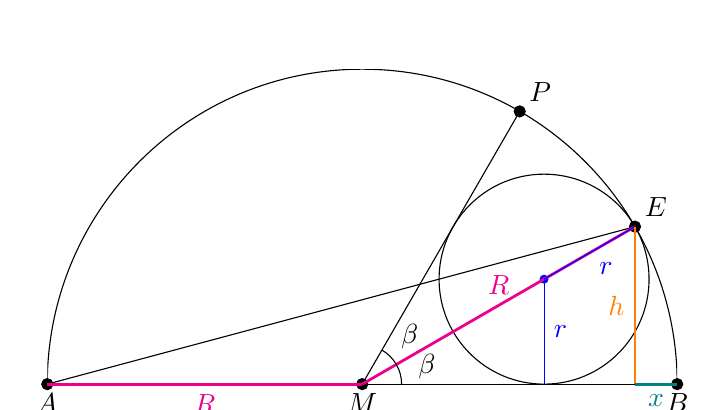
\begin{tikzpicture}[scale=4]
		% Koordinaten
		\coordinate (m) at (0,0);
		\coordinate (a) at (-1,0);
		\coordinate (b) at (1,0);
		\coordinate (p) at (0.5,0.866);
		\coordinate (e) at (0.866,0.5);
		\coordinate (kam) at (0.57732,0.33335);

		% Halbkreis
		\begin{scope}
			\clip (a) rectangle (1,1);
			\draw[black] (m) circle(1);
			\draw[black] (a) -- (b);
		\end{scope}

		% Kreis k_a
		\draw (kam) circle(0.33334);

		% Punkte
		\filldraw[black] (m) circle (0.5pt) node[anchor=north]{$M$};
		\filldraw[black] (a) circle (0.5pt) node[anchor=north]{$A$};
		\filldraw[black] (b) circle (0.5pt) node[anchor=north]{$B$};
		\filldraw[black] (p) circle (0.5pt) node[anchor=south west]{$P$};
		\filldraw[black] (e) circle (0.5pt) node[anchor=south west]{$E$};
		\filldraw[blue] (kam) circle (0.35pt);

		% Linien
		\draw[black] (a) -- (e);
		\draw[black] (m) -- (p);
		\draw[magenta, line width=1pt] (m) -- (e) node[midway,above]{$R$};
		\draw[magenta, line width=1pt] (a) -- (m) node[midway,below]{$R$};
		\draw[blue] (kam) -- (e) node[midway,below right]{$r$};
		\draw[blue] (kam) -- (0.57732,0) node[midway,right]{$r$};
		\draw[orange, line width=1pt] (e) -- (0.866,0) node[midway,left]{$h$};
		\draw[teal, line width=1pt] (b) -- (0.866,0) node[midway,below]{$x$};

		% Winkel
		\pic [draw,"$\beta$",angle eccentricity=1.7]{angle = b--m--e};
		\pic [draw,"$\beta$",angle eccentricity=1.7]{angle = e--m--p};
	\end{tikzpicture}
\end{center}

\begin{align*}
	m_{AE} &= \frac{\Delta y}{\Delta x} = \frac{h}{2R-x} \\
	\frac{h}{R} = \frac{r}{R-r} \leftrightarrow h &= \frac{Rr}{R-r} \tag{1}
\end{align*}

\begin{align*}
	\sin\beta &= \frac{\text{Gegenkathete}}{\text{Hypotenuse}} \\ 
	\sin\beta &= \frac{r}{R-r} \\
	r &= R \sin\beta - r \sin\beta \\
	r + r \sin\beta &= R \sin\beta \\
	r(1+\sin\beta) &= R \sin\beta \\
	r &= \frac{R \sin\beta}{1 + \sin\beta} \tag{2}
\end{align*}

\begin{samepage}
	\begin{center}
		\begin{tikzpicture}[scale=13]
			% Kreissektor mit 20°
			\draw[black] (m) -- (0:1) arc(0:20:1) -- cycle;

			% Punkte
			\coordinate (m) at (0,0);
			\coordinate (b) at (1,0);
			\coordinate (b2) at (0.93969,0.34202);
			\coordinate (p) at (0.98481,0.17365);
			\coordinate (p_) at (0.98481,0);
			\coordinate (kam) at (0.83896,0.14772);
			\coordinate (kam_side) at (0.98481,0.14772);

			\filldraw[black] (m) circle (0.25pt) node[anchor=east]{$M$};
			\filldraw[black] (p) circle (0.25pt) node[anchor=south west]{$P$};

			% Linien
			\draw[orange, line width=1pt] (p) -- (0.98481,0) node[midway,right]{$h$};
			\draw[magenta, line width=1pt] (m) -- (b2) node[midway,above left]{$R$};
			\draw[violet] (kam) -- (p) node[midway,above]{$r$};
			\draw[violet, line width=1pt] (kam) -- (0.83896,0) node[midway,left]{$r$};
			\draw[blue, line width=1pt] (m) -- (p_) node[midway,below]{$R_0$};
			\draw[teal, line width=1pt] (p_) -- (b) node[midway,below]{$x$};
			\draw[cyan, line width=1pt] (kam) -- (kam_side) node[midway,below]{$b$};
			\draw[black] (m) -- (p);

			% Kreis k_a
			\draw (kam) circle(0.14812);

			% Winkel
			\pic [draw,"$\beta$",angle eccentricity=2.6]{angle = b--m--b2};
			\pic [draw,"\tiny$\beta$\normalsize",angle eccentricity=2]{angle = kam_side--kam--p};
		\end{tikzpicture}
	\end{center}

	\begin{align*}
		\frac{R_0}{h} &= \frac{R_0-b}{r} \\
		r R_0 &= h R_0 - hb \\
		r R_0 - h R_0 &= -hb \\
		R_0 (r-h) &= -hb \\
		R_0 &= \frac{-hb}{r-h}
	\end{align*}
	Mit $ \cos\beta = \frac{b}{r} \Leftrightarrow b = r \cos\beta $ und $(1)$:
	\begin{align*}
		R_0 &= \frac{\frac{-Rr}{R-r}*r \cos\beta}{r-\frac{Rr}{R-r}} \\
		&= \frac{\left(\frac{-Rr}{R-r}*r \cos\beta\right)}{\left(\frac{(R-r)r}{R-r}-\frac{Rr}{R-r}\right)} \\
		&= \frac{\left(\frac{-Rr}{R-r}*r \cos\beta\right)}{\left(\frac{Rr-r^2-Rr}{R-r}\right)} \\
		&= \frac{\left(\frac{-Rr^2 \cos\beta}{R-r}\right)}{\left(-\frac{r^2}{R-r}\right)} \\
		&= \frac{-Rr^2 \cos\beta * (R-r)}{-(R-r)r^2} \\
		R_0 &= R \cos\beta
	\end{align*}

	\begin{align*}
		R_0 + x &= R \\
		x &= R - R_0 \\
		&= R - R \cos\beta \tag{3}
	\end{align*}
\end{samepage} \goodbreak

\begin{samepage}
	\begin{align*}
		m_{AE} &= \frac{h}{2R - x} \\
	\end{align*}
	Mit $(1)$ und $(3)$: \nopagebreak
	\begin{align*}
		m_{AE} &= \frac{\frac{Rr}{R-r}}{2R - (R-R \cos\beta)} \\
		&= \frac{\frac{Rr}{R-r}}{R+R \cos\beta} \\
		&= \frac{Rr}{(R-r)(R+R \cos\beta)} \\
		&= \frac{r}{(R-r)(1+\cos\beta)}
	\end{align*}
	Mit $(2)$: \nopagebreak
	\begin{align*}
		m_{AE} &= \frac{\frac{R \sin\beta}{1+\sin\beta}}{(R-r)(1+\cos\beta)} \\
		&= \frac{R \sin\beta}{(R-r)(1+\cos\beta)(1+\sin\beta)} \\
		&= \frac{R \sin\beta}{(R-\frac{R \sin\beta}{1+\sin\beta})(1+\cos\beta)(1+\sin\beta)} \\
		&= \frac{R \sin\beta}{(\frac{R(1+\sin\beta)}{1+\sin\beta}-\frac{R \sin\beta}{1+\sin\beta})(1+\cos\beta)(1+\sin\beta)} \\
		&= \frac{R \sin\beta}{(\frac{R(1+\sin\beta) - R\sin\beta}{1+\sin\beta})(1+\cos\beta)(1+\sin\beta)} \\
		&= \frac{R \sin\beta}{(\frac{R+R\sin\beta-R\sin\beta}{1+\sin\beta})(1+\cos\beta)(1+\sin\beta)} \\
		&= \frac{R \sin\beta}{(\frac{R}{1+\sin\beta})(1+\cos\beta)(1+\sin\beta)} \\
		&= \frac{\sin\beta}{(\frac{1}{1+\sin\beta})(1+\cos\beta)(1+\sin\beta)} \\
		&= \frac{(\sin\beta)(1+\sin\beta)}{(1+\sin\beta)(1+\cos\beta)} \\
		m_{AE} &= \frac{\sin\beta}{1+\cos\beta}
	\end{align*}
\end{samepage}

\pagebreak

\subsection[]{Herleitung von $m_{CD}$}
Hierfür relevante Punkte und Strecken:

\begin{center}
	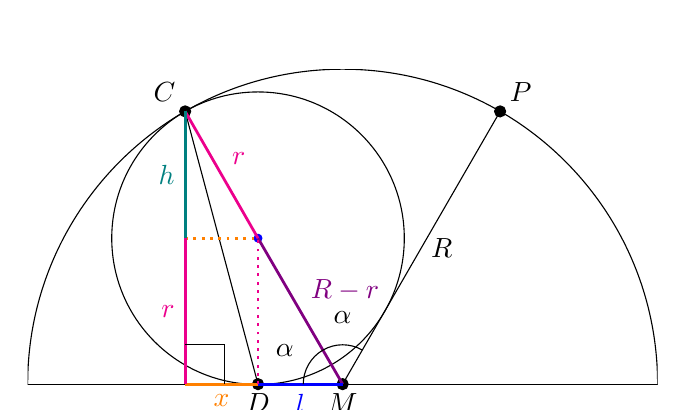
\begin{tikzpicture}[scale=4]
		% Koordinaten
		\coordinate (m) at (0,0);
		\coordinate (a) at (-1,0);
		\coordinate (b) at (1,0);
		\coordinate (p) at (0.5,0.866);
		\coordinate (c) at (-0.5,0.866);
		\coordinate (c_) at (-0.5,0);
		\coordinate (d) at (-0.26864,0);
		\coordinate (kbm) at (-0.26864,0.46335);
		\coordinate (kbm_side) at (-0.5,0.46335);

		% Kreis k_b
		\draw (kbm) circle(0.46441);

		% Halbkreis
		\begin{scope}
			\clip (a) rectangle (1,1);
			\draw[black] (m) circle(1);
			\draw[black] (a) -- (b);
		\end{scope}

		% Punkte
		\filldraw[black] (m) circle (0.5pt) node[anchor=north]{$M$};
		\filldraw[black] (d) circle (0.5pt) node[anchor=north]{$D$};
		\filldraw[black] (p) circle (0.5pt) node[anchor=south west]{$P$};
		\filldraw[black] (c) circle (0.5pt) node[anchor=south east]{$C$};
		\filldraw[blue] (kbm) circle (0.35pt);

		% Linien
		\draw[black] (m) -- (p) node[midway,right]{$R$};
		\draw[black] (c) -- (d);

		\draw[violet, line width=1pt] (m) -- (kbm) node[midway,above right]{$R-r$};
		\draw[magenta, line width=1pt] (kbm) -- (c) node[midway,above right]{$r$};
		\draw[blue, line width=1pt] (m) -- (d) node[midway,below]{$l$};
		\draw[orange, line width=1pt] (c_) -- (d) node[midway,below]{$x$};
		\draw[orange, dotted, line width=1pt] (kbm_side) -- (kbm) node[midway,below]{};
		\draw[magenta, line width=1pt] (c_) -- (kbm_side) node[midway,left]{$r$};
		\draw[magenta, dotted, line width=1pt] (d) -- (kbm) node[midway,left]{};
		\draw[teal, line width=1pt] (kbm_side) -- (c) node[midway, left]{$h$};

		% Winkel
		\pic [draw,"$\alpha$",angle eccentricity=1.7]{angle = p--m--c};
		\pic [draw,"$\alpha$",angle eccentricity=1.7]{angle = c--m--a};
		\pic [draw,angle eccentricity=1]{right angle = c--c_--m};
	\end{tikzpicture}
\end{center}

\begin{align*}
	m_{CD} &= \frac{\Delta y}{\Delta x} = \frac{h+r}{-x}
\end{align*}

\begin{align*}
	\textcolor{violet}{(R-r)}^2 &= \textcolor{magenta}{r}^2+\textcolor{blue}{l}^2 \\
	l &= \sqrt{(R-r)^2-r^2} \\
	&= \sqrt{R(R-2r)} \tag{1}
\end{align*}

\begin{align*}
	\sin\alpha &= \frac{\text{Gegenkathete}}{\text{Hypotenuse}} \\
	\sin\alpha &= \frac{ \textcolor{magenta}{r} }{ \textcolor{violet}{R-r} } \\
	r &= R\sin\alpha - r\sin\alpha \\
	r(1+\sin\alpha) &= R\sin\alpha \\
	r &= \frac{R\sin\alpha}{1+\sin\alpha} \tag{2}
\end{align*}

\begin{align*}
	\textcolor{teal}{h}^2 + \textcolor{orange}{x}^2 &= \textcolor{magenta}{r}^2 \\
	h &= \sqrt{r^2-x^2} \tag{3}
\end{align*}

\begin{samepage}
	\begin{align*}
		\frac{l}{r} &= \frac{l+x}{r+h} \\
		\text{Mit (3):} \\
		\frac{l}{r} &= \frac{l+x}{r+\sqrt{r^2-x^2}} \\
		(r+\sqrt{r^2-x^2})l &= r(l+x) \\
		rl + l\sqrt{r^2-x^2} &= rl+rx \\
		l\sqrt{r^2-x^2} &= rx \\
		l^2(r^2-x^2) &= r^2 x^2 \\
		l^2 r^2 - l^2 x^2 &= r^2 x^2 \\
		r^2 x^2 + l^2 x^2 &= l^2 r^2 \\
		x^2 (r^2+l^2) &= l^2 r^2 \\
		x^2 &= \frac{l^2 r^2}{r^2 + l^2} \\
		x &= \frac{lr}{\sqrt{r^2+l^2}} \\
		&= \frac{lr}{R-r} \\
		\text{Mit (1):} \\
		&= \frac{\sqrt{R(R-2r)}r}{R-r} \\
		\text{Mit (2):} \\
		&= \frac{\sqrt{R(R-2\frac{R\sin\alpha}{1+\sin\alpha})}\frac{R\sin\alpha}{1+\sin\alpha}}{R-\frac{R\sin\alpha}{1+\sin\alpha}} \\
		&= \frac{\sqrt{R(R-2\frac{R\sin\alpha}{1+\sin\alpha})}\frac{R\sin\alpha}{1+\sin\alpha}}{\frac{R}{1+\sin\alpha}} \\
		&= \frac{R\sqrt{\frac{1-\sin\alpha}{1+\sin\alpha}}\frac{\sin\alpha}{1+\sin\alpha}}{\frac{1}{1+\sin\alpha}} \\
		x &= R\sin\alpha\sqrt{\frac{1-\sin\alpha}{1+\sin\alpha}} \tag{4}
	\end{align*}
\end{samepage} \goodbreak

\begin{samepage}
	Weitergehend von $(3)$, mit $(2)$ und $(4)$: \nopagebreak
	\begin{align*}
		h &= \sqrt{r^2-x^2} \\
		&= \sqrt{\left(\frac{R\sin\alpha}{1+\sin\alpha}\right)^2 - \left(R\sin\alpha\sqrt{\frac{1-\sin\alpha}{1+\sin\alpha}}\right)^2} \\
		&= \sqrt{\frac{(R\sin\alpha)^2}{(1+\sin\alpha)^2} - \frac{(R\sin\alpha)^2(1-\sin\alpha)}{1+\sin\alpha}} \\
		&= \sqrt{\frac{(R\sin\alpha)^2}{(1+\sin\alpha)^2} - \frac{(R\sin\alpha)^2(1-\sin\alpha)(1+\sin\alpha)}{(1+\sin\alpha)^2}} \\
		&= \frac{\sqrt{(R\sin\alpha)^2(1-(1-\sin\alpha)(1+\sin\alpha))}}{1+\sin\alpha} \\
		&= R\sin\alpha \, \frac{\sqrt{1-(1-\sin\alpha)(1+\sin\alpha)}}{1+\sin\alpha} \\
		&= R\sin\alpha \, \frac{\sqrt{1-(1-\sin^2\alpha)}}{1+\sin\alpha} \\
		h &= R\sin\alpha \, \frac{\sin\alpha}{1+\sin\alpha} \tag{$3^\prime$}
	\end{align*}
\end{samepage} \goodbreak

\begin{samepage}
	Mit $(2)$, $(3^\prime)$ und $(4)$: \nopagebreak
	\begin{align*}
		m_{CD} &= \frac{h+r}{-x} \\
		&= \frac{R\sin\alpha \frac{\sin\alpha}{1+\sin\alpha} + \frac{R\sin\alpha}{1+\sin\alpha}}{-R\sin\alpha\sqrt{\frac{1-\sin\alpha}{1+\sin\alpha}}} \\
		&= \frac{\frac{\sin\alpha+1}{1+\sin\alpha}}{-\sqrt{\frac{1-\sin\alpha}{1+\sin\alpha}}} \\
		&= -\sqrt{\frac{1+\sin\alpha}{1-\sin\alpha}} \\
		&= -\frac{\sqrt{1+\sin\alpha}}{\sqrt{1-\sin\alpha}} \\
		&= -\frac{\sqrt{1+\sin\alpha}\sqrt{1+\sin\alpha}}{\sqrt{1-\sin\alpha}\sqrt{1+\sin\alpha}} \\
		&= -\frac{1+\sin\alpha}{\sqrt{1 - \sin^2\alpha}} \\
		&= -\frac{\sin\alpha+1}{\sqrt{\cos^2\alpha}} \\[15pt]
		&= -\frac{\sin\alpha+1}{\cos\alpha}
	\end{align*}
\end{samepage}

\pagebreak
Für die Winkel $\alpha$ und $\beta$ gilt:

\begin{center}
	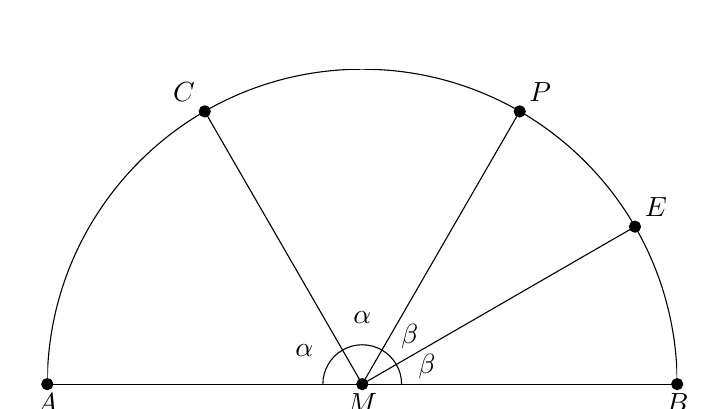
\begin{tikzpicture}[scale=4]
		% Punkte
		\coordinate (m) at (0,0);
		\coordinate (a) at (-1,0);
		\coordinate (b) at (1,0);
		\coordinate (p) at (0.5,0.866);
		\coordinate (c) at (-0.5,0.866);
		\coordinate (e) at (0.866,0.5);

		% Halbkreis
		\begin{scope}
			\clip (a) rectangle (1,1);
			\draw[black] (m) circle(1);
			\draw[black] (a) -- (b);
		\end{scope}

		% Punkte
		\filldraw[black] (m) circle (0.5pt) node[anchor=north]{$M$};
		\filldraw[black] (a) circle (0.5pt) node[anchor=north]{$A$};
		\filldraw[black] (b) circle (0.5pt) node[anchor=north]{$B$};
		\filldraw[black] (p) circle (0.5pt) node[anchor=south west]{$P$};
		\filldraw[black] (c) circle (0.5pt) node[anchor=south east]{$C$};
		\filldraw[black] (e) circle (0.5pt) node[anchor=south west]{$E$};

		% Linien
		\draw[black] (m) -- (p);
		\draw[black] (m) -- (c);
		\draw[black] (m) -- (e);

		% Winkel
		\pic [draw,"$\alpha$",angle eccentricity=1.7]{angle = p--m--c};
		\pic [draw,"$\alpha$",angle eccentricity=1.7]{angle = c--m--a};
		\pic [draw,"$\beta$",angle eccentricity=1.7]{angle = b--m--e};
		\pic [draw,"$\beta$",angle eccentricity=1.7]{angle = e--m--p};
	\end{tikzpicture}
\end{center}
\begin{align*}
	2\beta + 2\alpha &= \ang{180} \\
	\alpha &= \ang{90} - \beta \\
	\sin\alpha &= \sin(\ang{90} - \beta) = \cos\beta \\
	\cos\alpha &= \cos(\ang{90} - \beta) = \sin\beta \\
\end{align*}
So lässt sich $m_{CD}$ anders ausdrücken:
\begin{align*}
	m_{CD} &= -\frac{\sin\alpha+1}{\cos\alpha} \\
	&= -\frac{\cos\beta+1}{\sin\beta} \\
	m_{AE} &= \frac{\sin\beta}{\cos\beta+1}
\end{align*}

Somit gilt $ m_{CD} = -\frac{1}{m_{AE}} $, und damit auch $CD \perp AE$.

\pagebreak
\section[]{Aufgabe 4}
In allen folgenden Diagrammen steht eine gestrichelte Linie für eine Symmetrieachse, blau und rot markierte Felder sind ausgemalt, wobei der Anfänger die Farbe blau hat. \\[10pt]
Läuft das Spiel zuletzt auf eine $2\times2$-Ecke hinaus, verliert der Spieler, der zuerst in dieses Feld malen muss: \\
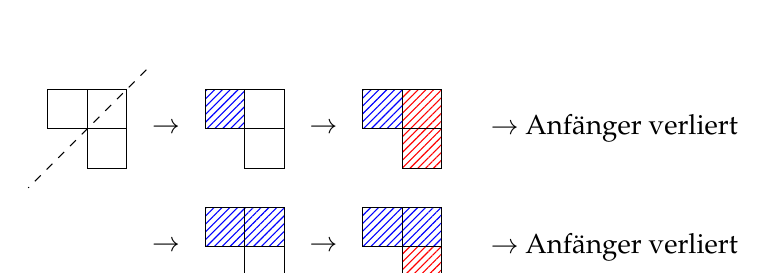
\begin{tikzpicture}[y=-0.5cm,x=0.5cm]
	\newcommand\Square{+(-0.5,-0.5) rectangle +(0.5,0.5)}
	\newcommand\RSquare{[pattern={Lines[angle=45,distance=2]}, pattern color=blue] +(-0.5,-0.5) rectangle +(0.5,0.5) }
	\newcommand\ESquare{[pattern={Lines[angle=45,distance=2]}, pattern color=red] +(-0.5,-0.5) rectangle +(0.5,0.5) }

	\draw (1,1) \Square;
	\draw (2,1) \Square;
	\draw (2,2) \Square;
	\draw [dashed] (3,0) -- (0,3);
	
	\node at (3.5,1.5) {$\rightarrow$};
	\draw (5,1) \RSquare;
	\draw (6,1) \Square;
	\draw (6,2) \Square;
	\node at (7.5,1.5) {$\rightarrow$};
	\draw (9,1) \RSquare;
	\draw (10,1) \ESquare;
	\draw (10,2) \ESquare;
	\node[anchor=west] at (11.5,1.5) {$\rightarrow$ Anfänger verliert};

	\node at (3.5,4.5) {$\rightarrow$};
	\draw (5,4) \RSquare;
	\draw (6,4) \RSquare;
	\draw (6,5) \Square;
	\node at (7.5,4.5) {$\rightarrow$};
	\draw (9,4) \RSquare;
	\draw (10,4) \RSquare;
	\draw (10,5) \ESquare;
	\node[anchor=west] at (11.5,4.5) {$\rightarrow$ Anfänger verliert};
\end{tikzpicture}
\\ Basierend darauf gilt dies auch für eine Ecke, die in beide Dimensionen beliebig viele Felder größer ist. Derjenige, der nicht anfängt, kopiert exakt die Menge an ausgemalten Feldern des Anfängers ($P$) auf der anderen Kante und zwingt den anfangenden Spieler in eine weitere kleinere $p\times p$-Ecke (dargestellt durch Orange):\\
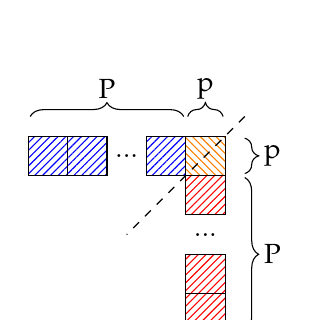
\begin{tikzpicture}[y=-0.5cm,x=0.5cm]
	\newcommand\Square{+(-0.5,-0.5) rectangle +(0.5,0.5)}
	\newcommand\Circle{+(0, 0) circle (0.35)}
	\newcommand\RSquare{[pattern={Lines[angle=45,distance=2]}, pattern color=blue] +(-0.5,-0.5) rectangle +(0.5,0.5) }
	\newcommand\ESquare{[pattern={Lines[angle=45,distance=2]}, pattern color=red] +(-0.5,-0.5) rectangle +(0.5,0.5) }
	\newcommand\RCircle{[pattern={Lines[angle=45,distance=2]}, pattern color=blue] +(0, 0) circle (0.35)}
	\newcommand\ECircle{[pattern={Lines[angle=45,distance=2]}, pattern color=red] +(0, 0) circle (0.35)}
	\newcommand\Corner{[pattern={Lines[angle=135,distance=2]}, pattern color=orange] +(-0.5,-0.5) rectangle +(0.5,0.5) }

	\draw (1,1) \RSquare;
	\draw (2,1) \RSquare;
	\node[anchor=center] at (3,1) {$...$};
	\draw (4,1) \RSquare;
	\draw (5,1) \Corner;
	\draw (5,2) \ESquare;
	\node[anchor=center] at (5,3) {$...$};
	\draw (5,4) \ESquare;
	\draw (5,5) \ESquare;
	\draw [dashed] (6,0) -- (3,3);

	\draw [decorate,decoration={brace,amplitude=5pt}] (0.55,0) -- (4.45,0) node[midway,yshift=1em]{P};
	\draw [decorate,decoration={brace,amplitude=5pt}] (4.55,0) -- (5.45,0) node[midway,yshift=1em]{p};
	
	\draw [decorate,decoration={brace,amplitude=5pt}] (6,0.55) -- (6,1.45) node[midway,xshift=1em]{p};
	\draw [decorate,decoration={brace,amplitude=5pt}] (6,1.55) -- (6,5.45) node[midway,xshift=1em]{P};

\end{tikzpicture} \\
Fährt Renate diese Strategie, kann sie Erhard irgendwann in eine $2\times2$-Ecke zwingen, in der er verliert, er hat also dann sicher verloren, wenn er in einer $p\times p$-Ecke beginnen muss. \\[10pt]
Läuft das Spiel auf eine "Hufeisenform" hinaus, verliert auch wieder der Spieler, der zuerst innerhalb dieser Form dran ist:

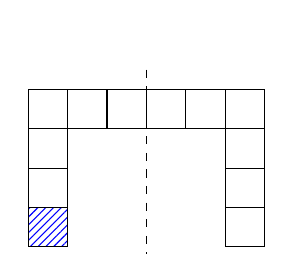
\begin{tikzpicture}[y=-0.5cm,x=0.5cm]
	\newcommand\Square{+(-0.5,-0.5) rectangle +(0.5,0.5)}
	\newcommand\RSquare{[pattern={Lines[angle=45,distance=2]}, pattern color=blue] +(-0.5,-0.5) rectangle +(0.5,0.5) }
	\newcommand\RRSquare{[fill=blue] +(-0.5,-0.5) rectangle +(0.5,0.5) }
	\newcommand\ESquare{[pattern={Lines[angle=45,distance=2]}, pattern color=red] +(-0.5,-0.5) rectangle +(0.5,0.5) }
	\newcommand\EESquare{[fill=red] +(-0.5,-0.5) rectangle +(0.5,0.5) }
	\newcommand\Corner{[pattern={Lines[angle=135,distance=2]}, pattern color=orange] +(-0.5,-0.5) rectangle +(0.5,0.5) }

	\draw (1,1) \Square;
	\draw (2,1) \Square;
	\draw (3,1) \Square;
	\draw (4,1) \Square;
	\draw (5,1) \Square;
	\draw (6,1) \Square;
	\draw (6,2) \Square;
	\draw (6,3) \Square;

	\draw (6,4) \Square;
	\draw (1,4) \RSquare;

	\draw (1,3) \Square;
	\draw (1,2) \Square;

	\draw [dashed] (3.5,0) -- (3.5,5);
\end{tikzpicture} $\rightarrow$ 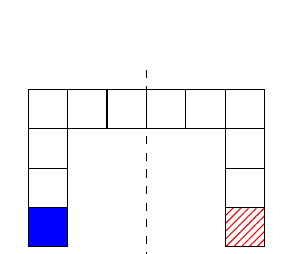
\begin{tikzpicture}[y=-0.5cm,x=0.5cm]
	\newcommand\Square{+(-0.5,-0.5) rectangle +(0.5,0.5)}
	\newcommand\RSquare{[pattern={Lines[angle=45,distance=2]}, pattern color=blue] +(-0.5,-0.5) rectangle +(0.5,0.5) }
	\newcommand\RRSquare{[fill=blue] +(-0.5,-0.5) rectangle +(0.5,0.5) }
	\newcommand\ESquare{[pattern={Lines[angle=45,distance=2]}, pattern color=red] +(-0.5,-0.5) rectangle +(0.5,0.5) }
	\newcommand\EESquare{[fill=red] +(-0.5,-0.5) rectangle +(0.5,0.5) }
	\newcommand\Corner{[pattern={Lines[angle=135,distance=2]}, pattern color=orange] +(-0.5,-0.5) rectangle +(0.5,0.5) }

	\draw (1,1) \Square;
	\draw (2,1) \Square;
	\draw (3,1) \Square;
	\draw (4,1) \Square;
	\draw (5,1) \Square;
	\draw (6,1) \Square;
	\draw (6,2) \Square;
	\draw (6,3) \Square;

	\draw (6,4) \ESquare;
	\draw (1,4) \RRSquare;

	\draw (1,3) \Square;
	\draw (1,2) \Square;

	\draw [dashed] (3.5,0) -- (3.5,5);
\end{tikzpicture} $\rightarrow$ 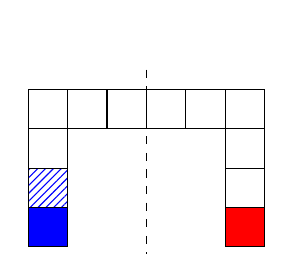
\begin{tikzpicture}[y=-0.5cm,x=0.5cm]
	\newcommand\Square{+(-0.5,-0.5) rectangle +(0.5,0.5)}
	\newcommand\RSquare{[pattern={Lines[angle=45,distance=2]}, pattern color=blue] +(-0.5,-0.5) rectangle +(0.5,0.5) }
	\newcommand\RRSquare{[fill=blue] +(-0.5,-0.5) rectangle +(0.5,0.5) }
	\newcommand\ESquare{[pattern={Lines[angle=45,distance=2]}, pattern color=red] +(-0.5,-0.5) rectangle +(0.5,0.5) }
	\newcommand\EESquare{[fill=red] +(-0.5,-0.5) rectangle +(0.5,0.5) }
	\newcommand\Corner{[pattern={Lines[angle=135,distance=2]}, pattern color=orange] +(-0.5,-0.5) rectangle +(0.5,0.5) }

	\draw (1,1) \Square;
	\draw (2,1) \Square;
	\draw (3,1) \Square;
	\draw (4,1) \Square;
	\draw (5,1) \Square;
	\draw (6,1) \Square;
	\draw (6,2) \Square;
	\draw (6,3) \Square;

	\draw (6,4) \EESquare;
	\draw (1,4) \RRSquare;

	\draw (1,3) \RSquare;
	\draw (1,2) \Square;

	\draw [dashed] (3.5,0) -- (3.5,5);
\end{tikzpicture} $\rightarrow$ 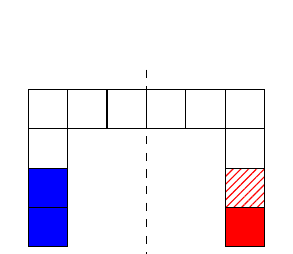
\begin{tikzpicture}[y=-0.5cm,x=0.5cm]
	\newcommand\Square{+(-0.5,-0.5) rectangle +(0.5,0.5)}
	\newcommand\RSquare{[pattern={Lines[angle=45,distance=2]}, pattern color=blue] +(-0.5,-0.5) rectangle +(0.5,0.5) }
	\newcommand\RRSquare{[fill=blue] +(-0.5,-0.5) rectangle +(0.5,0.5) }
	\newcommand\ESquare{[pattern={Lines[angle=45,distance=2]}, pattern color=red] +(-0.5,-0.5) rectangle +(0.5,0.5) }
	\newcommand\EESquare{[fill=red] +(-0.5,-0.5) rectangle +(0.5,0.5) }
	\newcommand\Corner{[pattern={Lines[angle=135,distance=2]}, pattern color=orange] +(-0.5,-0.5) rectangle +(0.5,0.5) }

	\draw (1,1) \Square;
	\draw (2,1) \Square;
	\draw (3,1) \Square;
	\draw (4,1) \Square;
	\draw (5,1) \Square;
	\draw (6,1) \Square;
	\draw (6,2) \Square;
	\draw (6,3) \ESquare;

	\draw (6,4) \EESquare;
	\draw (1,4) \RRSquare;

	\draw (1,3) \RRSquare;
	\draw (1,2) \Square;

	\draw [dashed] (3.5,0) -- (3.5,5);
\end{tikzpicture} $\rightarrow$ 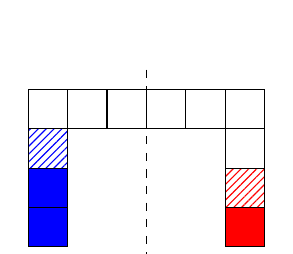
\begin{tikzpicture}[y=-0.5cm,x=0.5cm]
	\newcommand\Square{+(-0.5,-0.5) rectangle +(0.5,0.5)}
	\newcommand\RSquare{[pattern={Lines[angle=45,distance=2]}, pattern color=blue] +(-0.5,-0.5) rectangle +(0.5,0.5) }
	\newcommand\RRSquare{[fill=blue] +(-0.5,-0.5) rectangle +(0.5,0.5) }
	\newcommand\ESquare{[pattern={Lines[angle=45,distance=2]}, pattern color=red] +(-0.5,-0.5) rectangle +(0.5,0.5) }
	\newcommand\EESquare{[fill=red] +(-0.5,-0.5) rectangle +(0.5,0.5) }
	\newcommand\Corner{[pattern={Lines[angle=135,distance=2]}, pattern color=orange] +(-0.5,-0.5) rectangle +(0.5,0.5) }

	\draw (1,1) \Square;
	\draw (2,1) \Square;
	\draw (3,1) \Square;
	\draw (4,1) \Square;
	\draw (5,1) \Square;
	\draw (6,1) \Square;
	\draw (6,2) \Square;
	\draw (6,3) \ESquare;

	\draw (6,4) \EESquare;
	\draw (1,4) \RRSquare;

	\draw (1,3) \RRSquare;
	\draw (1,2) \RSquare;

	\draw [dashed] (3.5,0) -- (3.5,5);
\end{tikzpicture} $\rightarrow$ 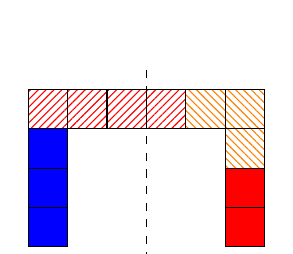
\begin{tikzpicture}[y=-0.5cm,x=0.5cm]
	\newcommand\Square{+(-0.5,-0.5) rectangle +(0.5,0.5)}
	\newcommand\RSquare{[pattern={Lines[angle=45,distance=2]}, pattern color=blue] +(-0.5,-0.5) rectangle +(0.5,0.5) }
	\newcommand\RRSquare{[fill=blue] +(-0.5,-0.5) rectangle +(0.5,0.5) }
	\newcommand\ESquare{[pattern={Lines[angle=45,distance=2]}, pattern color=red] +(-0.5,-0.5) rectangle +(0.5,0.5) }
	\newcommand\EESquare{[fill=red] +(-0.5,-0.5) rectangle +(0.5,0.5) }
	\newcommand\Corner{[pattern={Lines[angle=135,distance=2]}, pattern color=orange] +(-0.5,-0.5) rectangle +(0.5,0.5) }

	\draw (1,1) \ESquare;
	\draw (2,1) \ESquare;
	\draw (3,1) \ESquare;
	\draw (4,1) \ESquare;
	\draw (5,1) \Corner;
	\draw (6,1) \Corner;
	\draw (6,2) \Corner;
	\draw (6,3) \EESquare;

	\draw (6,4) \EESquare;
	\draw (1,4) \RRSquare;

	\draw (1,4) \Square;
	\draw (1,3) \RRSquare;
	\draw (1,2) \RRSquare;

	\draw [dashed] (3.5,0) -- (3.5,5);
\end{tikzpicture}
\\ Erhard findet sich nun in einer $p\times p$-Ecke und verliert. \\[10pt]
Renate hat nun für zwei verschiedene Größen von Feldern Strategien.
\begin{itemize}
	\item[Fall 1:] $n=m$
\end{itemize}
Hierfür beginnt Renate mit dem Ausmalen eines einzelnen Feldes E in einer Ecke. Erhard kann in seinem nächsten Zug nur bis zu $n-1$ Felder auf genau einer Kante ausmalen. Renate wird solange mit jedem ihrer Züge das Spielfeld symmetrisch zur Spiegelachse, die die Strecke zwischen E und der Ecke diagonal gegenüber von E ist (eingezeichnet als gestrichelte Linie), halten, bis sich Erhard als Anfänger in einer $p\times p$-Ecke findet und verliert. \\
Ab dem zweiten Diagramm macht pro Bild immer erst rot/Erhard einen Zug, dann blau/Renate: \\[10pt]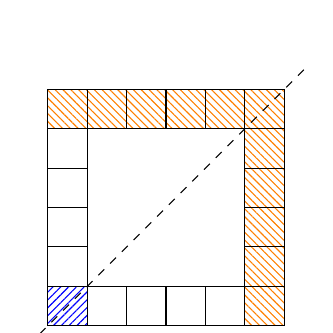
\begin{tikzpicture}[y=-0.5cm,x=0.5cm]
	\newcommand\Square{+(-0.5,-0.5) rectangle +(0.5,0.5)}
	\newcommand\Circle{+(0, 0) circle (0.35)}
	\newcommand\RSquare{[pattern={Lines[angle=45,distance=2]}, pattern color=blue] +(-0.5,-0.5) rectangle +(0.5,0.5) }
	\newcommand\ESquare{[pattern={Lines[angle=45,distance=2]}, pattern color=red] +(-0.5,-0.5) rectangle +(0.5,0.5) }
	\newcommand\RCircle{[pattern={Lines[angle=45,distance=2]}, pattern color=blue] +(0, 0) circle (0.35)}
	\newcommand\ECircle{[pattern={Lines[angle=45,distance=2]}, pattern color=red] +(0, 0) circle (0.35)}
	\newcommand\Corner{[pattern={Lines[angle=135,distance=2]}, pattern color=orange] +(-0.5,-0.5) rectangle +(0.5,0.5) }

	\draw (1,1) \Corner; 
	\draw (2,1) \Corner;
	\draw (3,1) \Corner;
	\draw (4,1) \Corner;
	\draw (5,1) \Corner;
	\draw (6,1) \Corner;
	\draw (6,2) \Corner;
	\draw (6,3) \Corner;
	\draw (6,4) \Corner;
	\draw (6,5) \Corner;
	\draw (6,6) \Corner;

	\draw (5,6) \Square;
	\draw (4,6) \Square;
	\draw (3,6) \Square;
	\draw (2,6) \Square;
	\draw (1,6) \RSquare;

	\draw (1,5) \Square;
	\draw (1,4) \Square;
	\draw (1,3) \Square;
	\draw (1,2) \Square;

	\draw [dashed] (7,0) -- (0,7);
\end{tikzpicture} $\rightarrow$ 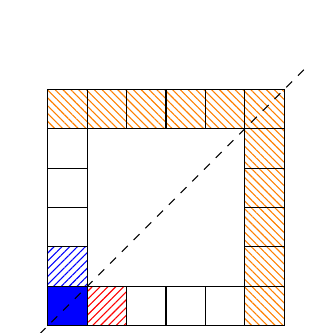
\begin{tikzpicture}[y=-0.5cm,x=0.5cm]
	\newcommand\Square{+(-0.5,-0.5) rectangle +(0.5,0.5)}
	\newcommand\Circle{+(0, 0) circle (0.35)}
	\newcommand\RSquare{[pattern={Lines[angle=45,distance=2]}, pattern color=blue] +(-0.5,-0.5) rectangle +(0.5,0.5) }
	\newcommand\RRSquare{[fill=blue] +(-0.5,-0.5) rectangle +(0.5,0.5) }
	\newcommand\ESquare{[pattern={Lines[angle=45,distance=2]}, pattern color=red] +(-0.5,-0.5) rectangle +(0.5,0.5) }
	\newcommand\EESquare{[fill=red] +(-0.5,-0.5) rectangle +(0.5,0.5) }
	\newcommand\Corner{[pattern={Lines[angle=135,distance=2]}, pattern color=orange] +(-0.5,-0.5) rectangle +(0.5,0.5) }

	\draw (1,1) \Corner;
	\draw (2,1) \Corner;
	\draw (3,1) \Corner;
	\draw (4,1) \Corner;
	\draw (5,1) \Corner;
	\draw (6,1) \Corner;
	\draw (6,2) \Corner;
	\draw (6,3) \Corner;
	\draw (6,4) \Corner;
	\draw (6,5) \Corner;
	\draw (6,6) \Corner;

	\draw (5,6) \Square;
	\draw (4,6) \Square;
	\draw (3,6) \Square;
	\draw (2,6) \ESquare;
	\draw (1,6) \RRSquare;

	\draw (1,5) \RSquare;
	\draw (1,4) \Square;
	\draw (1,3) \Square;
	\draw (1,2) \Square;

	\draw [dashed] (7,0) -- (0,7);
\end{tikzpicture} $\rightarrow$ 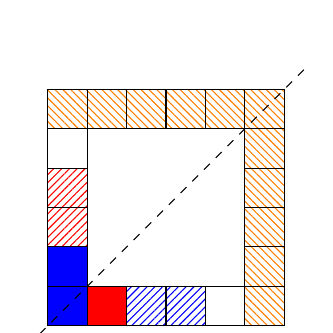
\begin{tikzpicture}[y=-0.5cm,x=0.5cm]
	\newcommand\Square{+(-0.5,-0.5) rectangle +(0.5,0.5)}
	\newcommand\Circle{+(0, 0) circle (0.35)}
	\newcommand\RSquare{[pattern={Lines[angle=45,distance=2]}, pattern color=blue] +(-0.5,-0.5) rectangle +(0.5,0.5) }
	\newcommand\RRSquare{[fill=blue] +(-0.5,-0.5) rectangle +(0.5,0.5) }
	\newcommand\ESquare{[pattern={Lines[angle=45,distance=2]}, pattern color=red] +(-0.5,-0.5) rectangle +(0.5,0.5) }
	\newcommand\EESquare{[fill=red] +(-0.5,-0.5) rectangle +(0.5,0.5) }
	\newcommand\Corner{[pattern={Lines[angle=135,distance=2]}, pattern color=orange] +(-0.5,-0.5) rectangle +(0.5,0.5) }

	\draw (1,1) \Corner;
	\draw (2,1) \Corner;
	\draw (3,1) \Corner;
	\draw (4,1) \Corner;
	\draw (5,1) \Corner;
	\draw (6,1) \Corner;
	\draw (6,2) \Corner;
	\draw (6,3) \Corner;
	\draw (6,4) \Corner;
	\draw (6,5) \Corner;
	\draw (6,6) \Corner;

	\draw (5,6) \Square;
	\draw (4,6) \RSquare;
	\draw (3,6) \RSquare;
	\draw (2,6) \EESquare;
	\draw (1,6) \RRSquare;

	\draw (1,5) \RRSquare;
	\draw (1,4) \ESquare;
	\draw (1,3) \ESquare;
	\draw (1,2) \Square;

	\draw [dashed] (7,0) -- (0,7);
\end{tikzpicture}
\\ Egal wieviele Felder Erhard in seinem nächsten Zug ausmalt, wird er in eine $p\times p$-Ecke (gezeichnet in Orange) gezwungen und verliert: \\
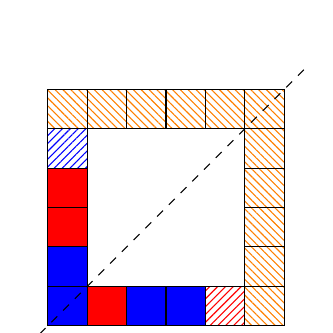
\begin{tikzpicture}[y=-0.5cm,x=0.5cm]
	\newcommand\Square{+(-0.5,-0.5) rectangle +(0.5,0.5)}
	\newcommand\Circle{+(0, 0) circle (0.35)}
	\newcommand\RSquare{[pattern={Lines[angle=45,distance=2]}, pattern color=blue] +(-0.5,-0.5) rectangle +(0.5,0.5) }
	\newcommand\RRSquare{[fill=blue] +(-0.5,-0.5) rectangle +(0.5,0.5) }
	\newcommand\ESquare{[pattern={Lines[angle=45,distance=2]}, pattern color=red] +(-0.5,-0.5) rectangle +(0.5,0.5) }
	\newcommand\EESquare{[fill=red] +(-0.5,-0.5) rectangle +(0.5,0.5) }
	\newcommand\Corner{[pattern={Lines[angle=135,distance=2]}, pattern color=orange] +(-0.5,-0.5) rectangle +(0.5,0.5) }

	\draw (1,1) \Corner;
	\draw (2,1) \Corner;
	\draw (3,1) \Corner;
	\draw (4,1) \Corner;
	\draw (5,1) \Corner;
	\draw (6,1) \Corner;
	\draw (6,2) \Corner;
	\draw (6,3) \Corner;
	\draw (6,4) \Corner;
	\draw (6,5) \Corner;
	\draw (6,6) \Corner;

	\draw (5,6) \ESquare;
	\draw (4,6) \RRSquare;
	\draw (3,6) \RRSquare;
	\draw (2,6) \EESquare;
	\draw (1,6) \RRSquare;

	\draw (1,5) \RRSquare;
	\draw (1,4) \EESquare;
	\draw (1,3) \EESquare;
	\draw (1,2) \RSquare;

	\draw [dashed] (7,0) -- (0,7);
\end{tikzpicture}
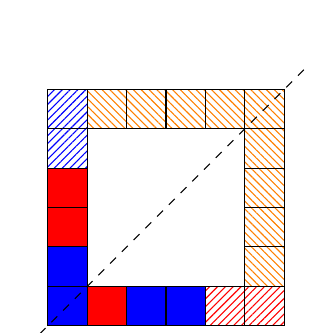
\begin{tikzpicture}[y=-0.5cm,x=0.5cm]
	\newcommand\Square{+(-0.5,-0.5) rectangle +(0.5,0.5)}
	\newcommand\Circle{+(0, 0) circle (0.35)}
	\newcommand\RSquare{[pattern={Lines[angle=45,distance=2]}, pattern color=blue] +(-0.5,-0.5) rectangle +(0.5,0.5) }
	\newcommand\RRSquare{[fill=blue] +(-0.5,-0.5) rectangle +(0.5,0.5) }
	\newcommand\ESquare{[pattern={Lines[angle=45,distance=2]}, pattern color=red] +(-0.5,-0.5) rectangle +(0.5,0.5) }
	\newcommand\EESquare{[fill=red] +(-0.5,-0.5) rectangle +(0.5,0.5) }
	\newcommand\Corner{[pattern={Lines[angle=135,distance=2]}, pattern color=orange] +(-0.5,-0.5) rectangle +(0.5,0.5) }

	\draw (1,1) \RSquare;
	\draw (2,1) \Corner;
	\draw (3,1) \Corner;
	\draw (4,1) \Corner;
	\draw (5,1) \Corner;
	\draw (6,1) \Corner;
	\draw (6,2) \Corner;
	\draw (6,3) \Corner;
	\draw (6,4) \Corner;
	\draw (6,5) \Corner;
	\draw (6,6) \ESquare;

	\draw (5,6) \ESquare;
	\draw (4,6) \RRSquare;
	\draw (3,6) \RRSquare;
	\draw (2,6) \EESquare;
	\draw (1,6) \RRSquare;

	\draw (1,5) \RRSquare;
	\draw (1,4) \EESquare;
	\draw (1,3) \EESquare;
	\draw (1,2) \RSquare;

	\draw [dashed] (7,0) -- (0,7);
\end{tikzpicture}

\begin{itemize}
	\item[Fall 2:] $n\neq m$
\end{itemize}
Hierbei malt Renate in ihrem ersten Zug eine der längeren Kanten komplett aus. So bleibt als Spielfeld noch eine "Hufeisenform" übrig. In diesem Hufeisen ist eine Seite um mindestens 2 Felder länger als die andere. Nach dem Beweis oben verliert der Anfänger (nach Renates Strategie also Erhard) in diesem Hufeisen auch (wie bereits oben gezeigt), Renate hat also hier auch eine sichere Gewinnstrategie.
\end{document}
